\chapter{分析方法}
\section{问题定义}
第一章中对本文所要解决的问题进行了简要介绍和定义。

考虑到补丁间不兼容的实质是因为在应用时和应用后出现了错误,可以具体将错误分为两类:

\begin{definition}
	兼容性错误——针对软件版本$v_1$的补丁$p_1$在应用到其他软件版本$v_2$时和之后可能出现的程序错误。主要分为两类:
	\begin{itemize}
		\item 语法错误:即出现语法结构上的错误。易由编译器发现。
		\item 语义错误:补丁$p_1$中的变更其语义和补丁$p_2=diff(v_1,v_2)$的变更语义出现冲突,较难发现。
	\end{itemize}
\end{definition}

因而,可见为了判定补丁间是否相容,我们主要需要判定两个补丁间是否存在语义上的冲突。

在实际的工作中,我们发现该问题可以拆分为若干个子问题。因而我们可以采用分治的办法去逐步解决这些子问题,最后将其组合起来,即是对第一章中所述的问题的解决方案。下面将对这些子问题及其解决方法分别阐述并定义之。

\subsection{补丁版本迁移}

【给出问题定义:对补丁进行版本迁移】
【给出补丁版本迁移的定义】

补丁程序是专门为某一版本的软件系统所设计,因而往往不能直接应用到其他版本的代码上,而且强行应用往往会出现很多错误。常见的问题可能包括:

\begin{enumerate}
	\item 补丁程序中所提及的行不在原位置。
	\item 补丁程序中所要删除的行其实已被删除,或者所要添加的行其实已被添加。
	\item 补丁程序中所提及的文件未找到。
\end{enumerate}

由于有这些可能的问题存在,导致我们无法直接将补丁程序应用到其他版本的补丁上。在这里我们先不考虑应用之后可能出现的语义错误,而尝试去解决可能出现的语法错误。因而这个问题可以如下定义之。

\begin{problem}
	\label {patch_reversion}
	由于补丁p针对版本$v_{1}$设计,当尝试将其应用到版本$v_{2}$上时,可能会出现程序语法结构上的错误。如何实现补丁的版本迁移,将p成功应用到版本$v_{2}$上,并且不会出现程序语法错误?
\end{problem}

为了解决这个问题,我们实际上可以采用版本控制系统的版本合并功能。

版本控制系统中经常需要将其他分支中的版本合并到当前分支中,为了解决不同版本之间可能存在的语法冲突,通常会采用三路归并算法(3-way merge)来对两个不同版本的代码进行合并,合并时以二者共同的祖先版本作为依据进行。

而我们所面临的问题也是类似的,由于$patch(p_1,v_1) = v_3$,为了将p1应用到版本v2上获得版本v4,我们可以采用类似的想法,将版本v3和版本v2进行合并即可。合并后我们就等于同时拥有了$p_1 = diff(v_1,v_3)$和$p_2 = diff(v_1,v_2)$这两个补丁中的变更。

这实际上也是现在软件开发过程中的常见手段。例如使用git作为版本控制系统时,为了修复某个功能性的bug,我们可以新建一个分支FixBug,然后切换到该分支进行漏洞修复,等到修补完毕后,再将该分支合并到主分支Master中即可。

该过程如图\ref{git_branch}所示。

\begin{figure}[H]	
	\centering
	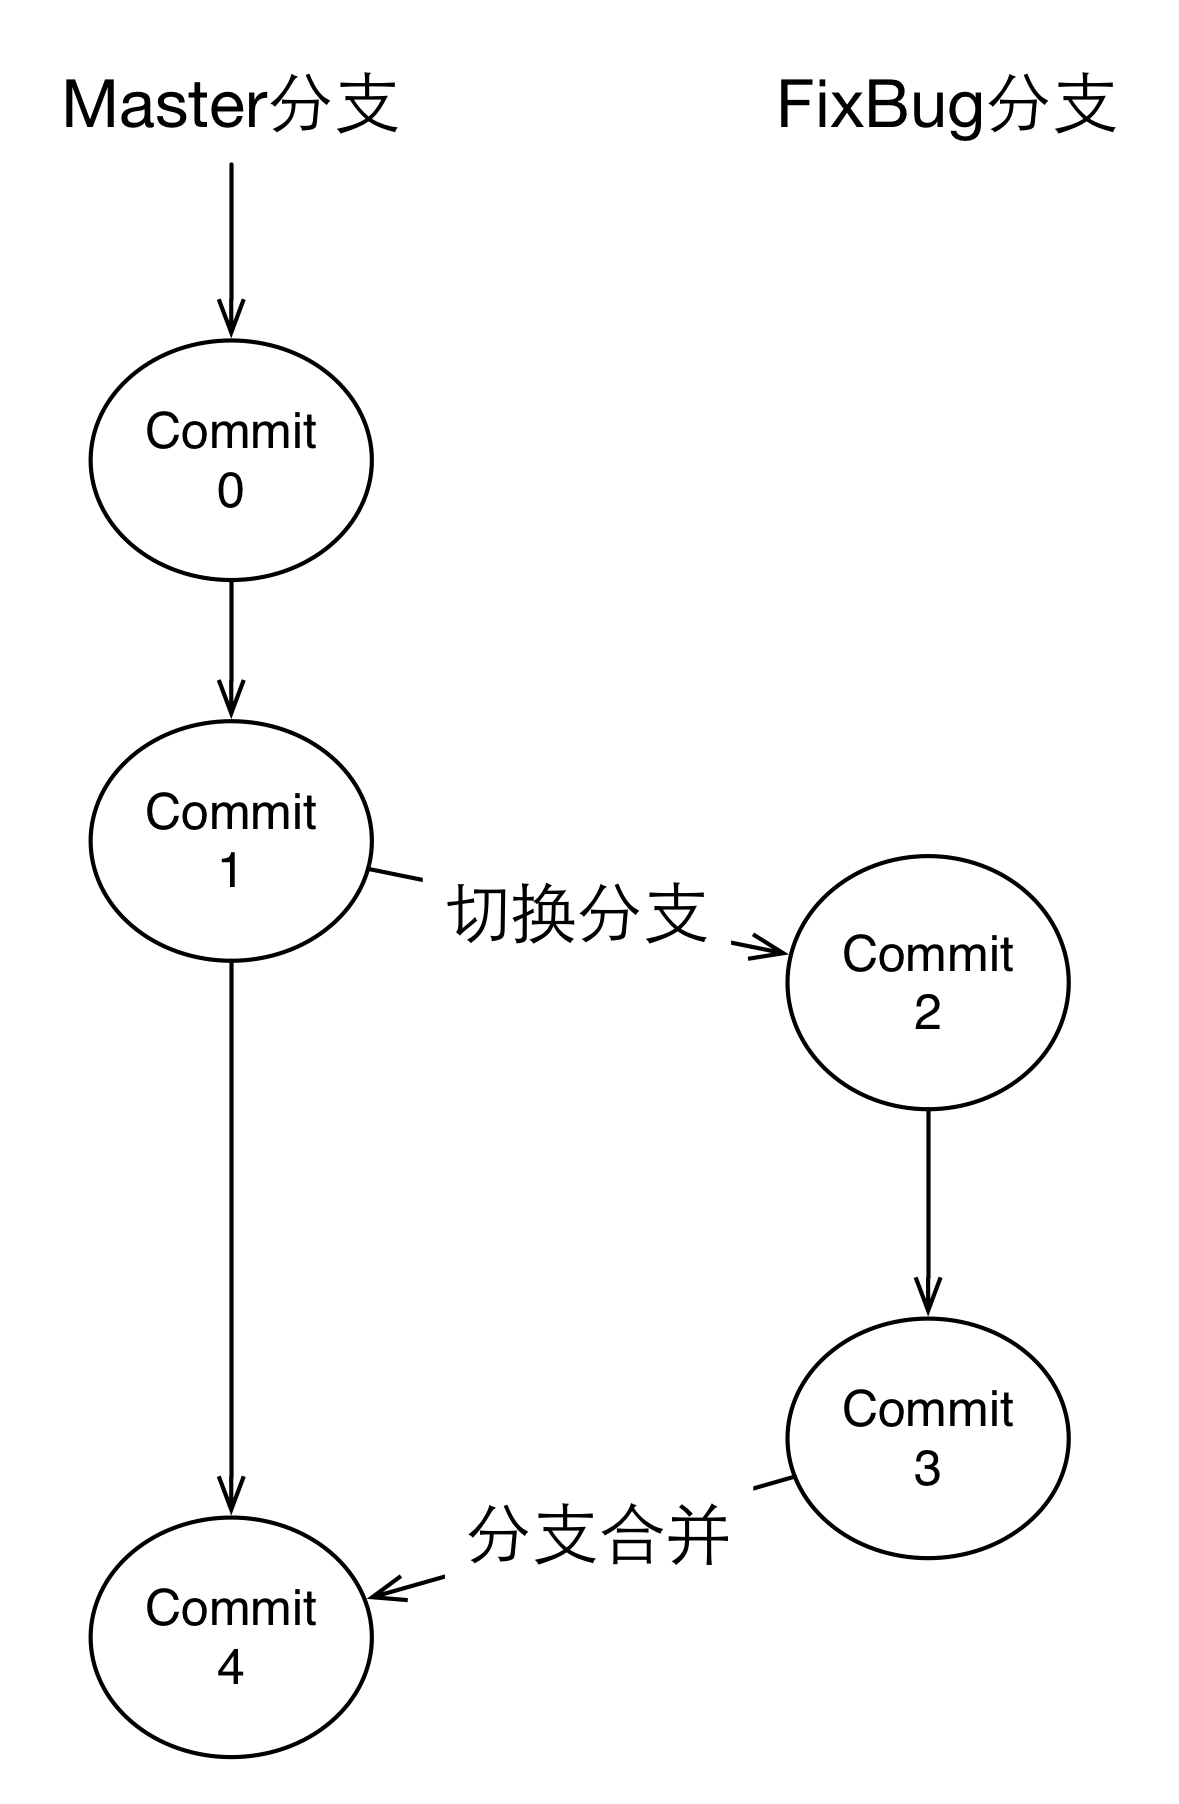
\includegraphics{chap03_git_branch}
	\caption {git分支切换与合并}	
	\label {git_branch}
\end{figure}

因而,我们可以将补丁版本迁移过程定义如下。

\begin{definition}
	补丁版本迁移——将原本为软件版本$v_1$所设计的补丁p修改为可以在另一软件版本$v_2$上使用的补丁,使得应用补丁之后不会出现程序语法结构错误。
\end{definition}

\subsection{语义影响范围分析}

【给出问题定义:分析出变更的语义影响范围】
【给出语义影响范围定义】

为了确定两个补丁之间是否存在互斥子集,我们需要从语义的角度入手。根据本文对互斥的定义,我们可以发现,我们主要需要从代码中挖掘中两类信息:
\begin{enumerate}
	\item 代码的变更集合,即两个版本之间代码的差异性。
	\item 变更的影响集合,即变更集合对代码中其他哪些部分会造成影响。
\end{enumerate}

在有了这两类集合之后,我们就可以界定出软件变更在语义层面上对代码的影响范围,我们可以将这整个过程称为语义影响范围分析(semantic impacted area analysis)。之后,我们可以通过比较两个补丁对代码的影响范围是否存在重叠来判定补丁间的互斥性。

因而,本节中的子问题主要在于如何界定软件变更对于程序的影响范围。


\begin{definition}
	软件变更(Software change)——对软件代码做出的修改。
	其中变更可以划分为三类不同的表示方法:
		\begin{itemize}
			\item 文本:只考虑程序代码在文本行上的变化。
			\item 语法:考虑程序代码在语法结构上的变化。
			\item 语义:考虑程序代码在语义层面上发生的变化。
		\end{itemize}
\end{definition}

\begin{definition}
	软件变更集合(Software change set)——补丁p中所涉及到的软件变更的集合。
\end{definition}

\begin{definition}
	程序结构——指程序的基础语法结构,包括类、方法、基本块、语句等不同级别。
\end{definition}

\begin{definition}
	影响范围(impated area)——在程序的某个限定范围中,直接或间接受到变更影响的程序结构集合。
\end{definition}

\begin{problem}
	\label {impacted_area}
	给定一个程序和他的变更集合,如何界定该变更集合对于其他程序结构的影响范围?
\end{problem}

事实上,可以将程序中受变更影响的部分划分为不同的粒度,从而获得不同程度的影响,我们考虑对面向对象的编程方法中的影响元素级别进行划分:

\begin{enumerate}
	\item 类:探讨变更对于其他类和对象的影响。对于面向对象的程序设计方法而言,这是最高级别的粒度。
	\item 方法:探讨变更对于其他方法的的影响。
	\item 基本块:探讨变更对于其他基本块的影响。
	\item 语句:探讨变更对于其他语句的影响。
\end{enumerate}

而所谓的影响范围也需要界定其粒度,不同层级的粒度显然会对语义影响范围分析的精度产生影响。

\begin{enumerate}
	\item 类间:考虑变更的影响可能延伸到其他类、对象。
	\item 方法间:考虑变更的影响可能延伸到其他方法内部。
	\item 方法内部:考虑变更的影响只在本方法的内部延伸。
\end{enumerate}

在实际情况中,不同级别的影响范围均可分别采用不同的影响元素级别。

通过语义影响范围分析,我们就可以从代码中挖掘出所需要的变更影响信息,从而可以进行后续的兼容性分析工作。

在实际应用中,语义影响范围分析主要由两类分析过程组成:
\begin{enumerate}
	\item 程序间差异性分析:获取两个软件版本间的差异性,获得结构化的软件变更信息。该分析过程即为$diff(v_1,v_2)$函数的具体实现。
	\item 变更影响分析:分析软件变更对软件其他部分是否存在影响,并找到受影响的集合。该分析过程即为$impact(p_1,v_1)$函数的具体实现。
\end{enumerate}


我们可以将整个分析过程定义为如下的函数:

\begin{definition}
	$ia(v_i,v_j) = impact(diff(v_i,v_j),v_i),i \subset \mathbb{N}, j \subset \mathbb{N}$
\end{definition}


\subsection{兼容性分析}

【给出问题定义:分析判定补丁的兼容性】
【给出兼容性的定义】

我们最后还是要落实到补丁兼容性的判定问题上来。在有了前面两个子问题的铺垫之后,我们就可以着手进行核心的补丁兼容性分析过程。因而该子问题可以定义如下。

\begin{problem}
	给定两个补丁和他们对代码的影响范围,问这两个补丁是否兼容,即不存在语义冲突?
\end{problem}

在有了软件变更的语义影响范围之后,我们可以通过简单地比较两个补丁对代码的影响范围是否存在重叠来判定其互斥性。

\begin{definition}
	影响范围的重叠——即两个影响范围间是否存在交集,如果存在交集,则重叠,反之亦然。
\end{definition}

显然,如果两个补丁对代码的影响范围不存在重叠,那么他们两者之间自然是兼容的,因为他们不仅本身的变更互不干涉,并且他们所影响到的程序结构也互不干涉。在这样的情况下,补丁是可以成功应用到其他版本上的代码,并且可以完成补丁本身的目标的。

如果影响范围发生了重叠,那么我们就可以认为补丁之间是不相容的,因为补丁所作的变更会对相同的程序结构产生影响。实际上这样的影响是否能够兼容需要人工的判定,因为在不同的情况下,他们可能是兼容的,也可能是不兼容的。而我们无法从代码中获取到足够的信息来进行这样的判定,需要人类对于变更的期望信息作为辅助。

我们可以将这个过程定义为如下类型的函数:

\begin{definition}
	$isCompatible(diff(v_2,v_1),diff(v_2,v_4)) :: Patch \rightarrow Patch \rightarrow Boolean$
\end{definition}

该函数接受两个补丁作为参数,并返回一个布尔类型的判定结果。

\section{应用场景}

本文中的主要问题在于如何判定一个针对给定程序版本的补丁,它是否能够应用于其他版本,并且与其兼容?为了使读者对这一问题更加清晰,我们可以考虑这样一个应用场景,并且有这样一些前提假设:

\begin{itemize}
	\item 某个团队正在对一软件进行开发工作,该软件已推出一个正式版$v_{1}$,现在正在进行$v_{2}$版本的开发。
	
	\item 该团队使用git作为版本管理系统,使用Github作为代码托管和团队协作工具。
	
	\item 该软件存在一个第三方开发的针对$v_{1}$版本的的补丁p,该补丁可以增强该软件的功能。
	
\end{itemize}

我们希望知道,该补丁p是否能够应用于正式版$v_{2}$,并且补丁p的原目标能够实现,且不影响软件版本$v_{2}$的正常功能?


\section{解决方案}
【介绍补丁兼容性分析方法的整体架构:补丁版本迁移、语义影响范围分析(程序差异性分析、程序变更影响分析)、补丁兼容性分析】

考虑上两节中所提到的应用场景和子问题划分,我们可以给出这样一个解决方案来解决整个兼容性问题的判定。该解决方案的整体架构如图\ref {structure}所示。

\begin{figure}[H]
	\centering
	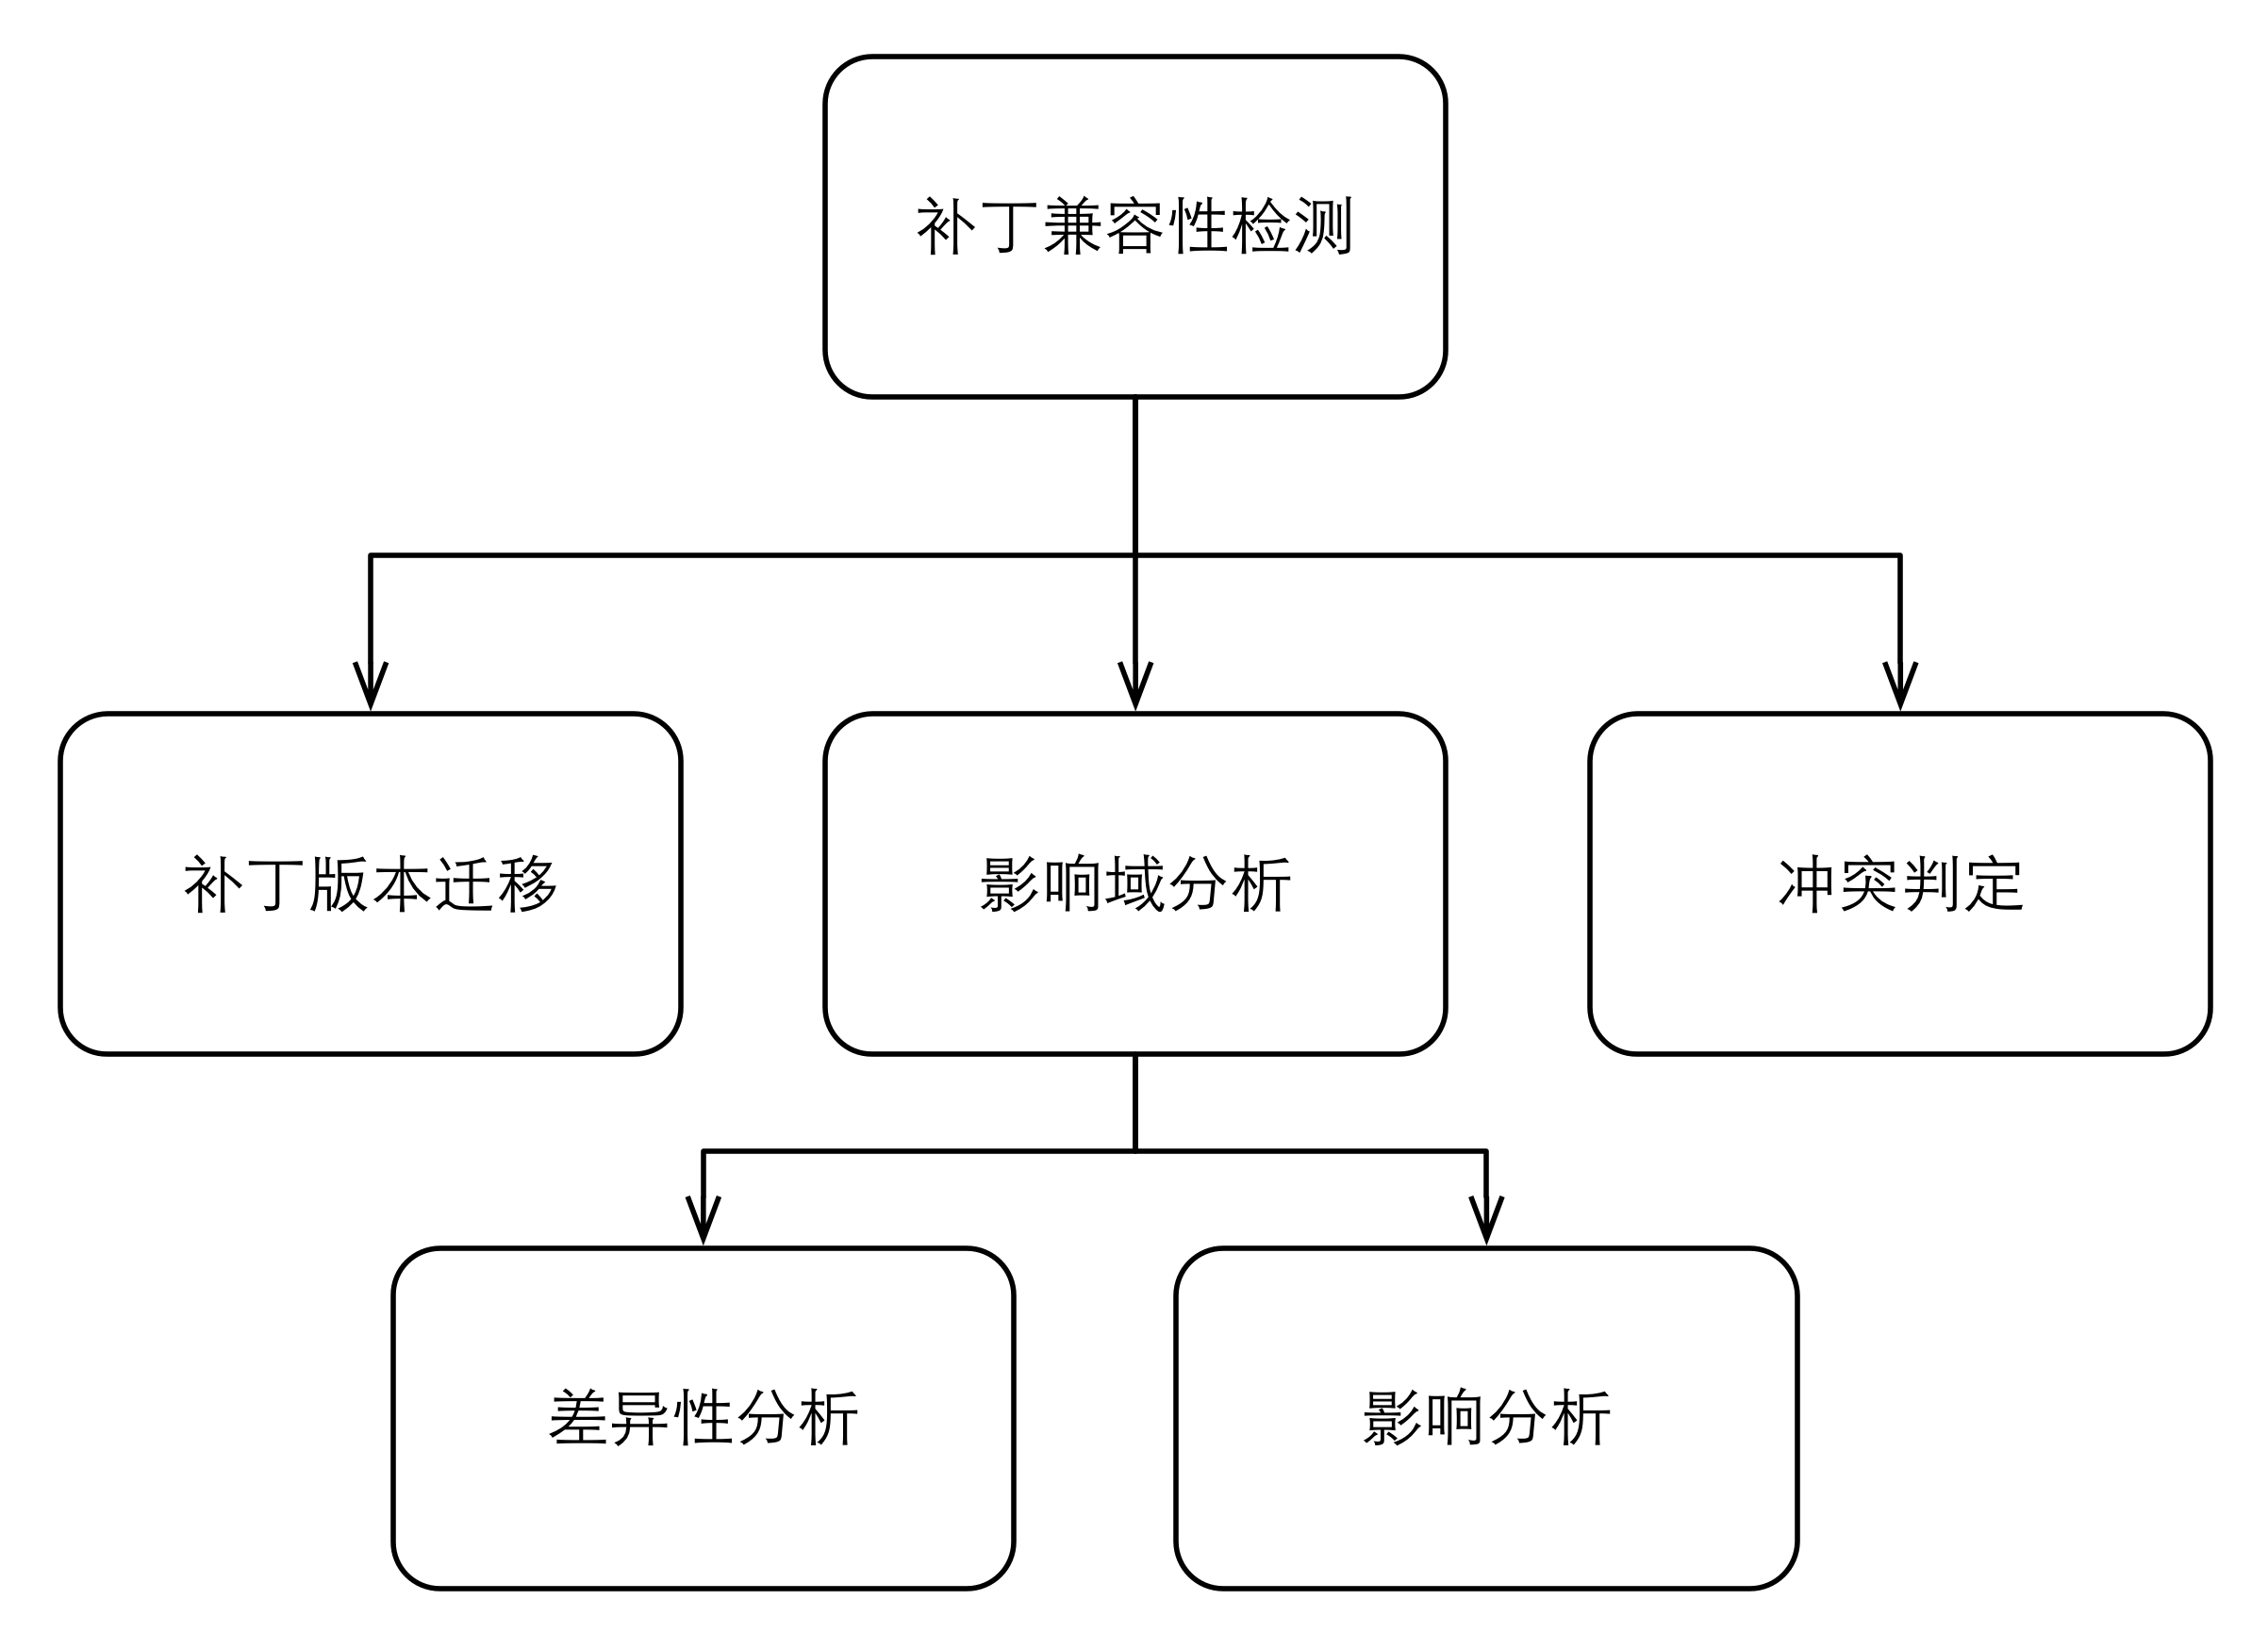
\includegraphics{chap03_structure}
	\caption {整体架构}	
	\label {structure}
\end{figure}

可见,问题\ref{compatible}的解决主要需要采用对应的解决方法分别解决三个子问题,最后将再将其组合起来即可,是一个应用了分治法的解决方案。

因此,根据上一节中分解出的各个子问题,我们可以给出一个整体的补丁兼容性分析流程图,如图\ref {all_flow}所示。

\begin{figure}[H]
	\centering
	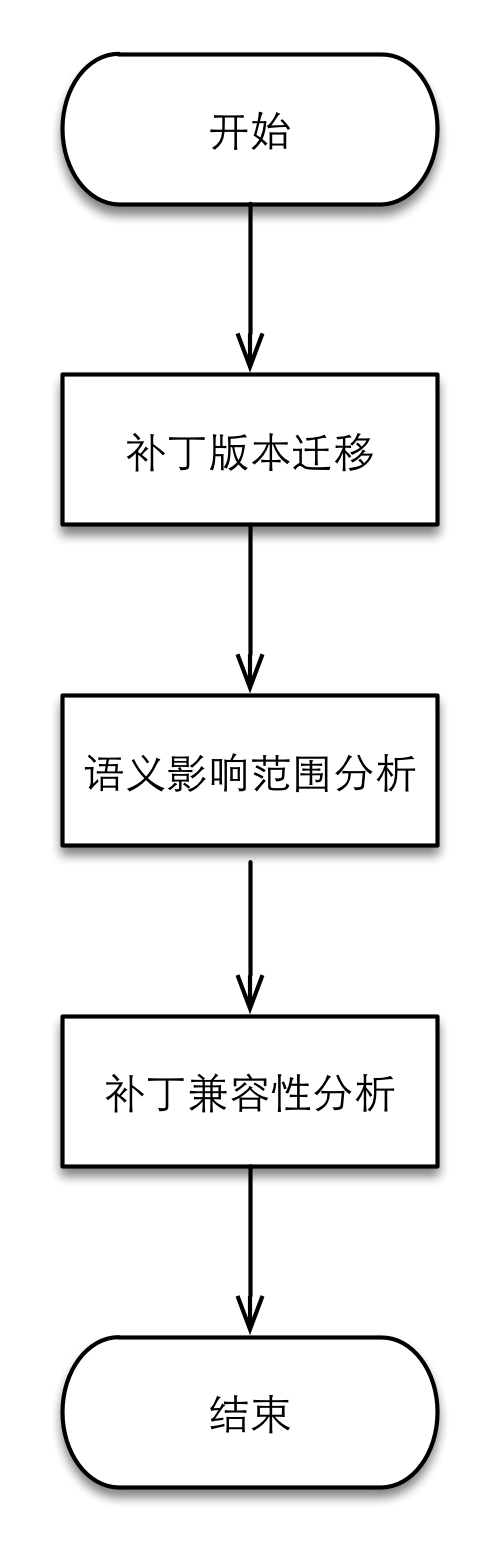
\includegraphics{chap03_abstract}
	\caption {整体流程}
	\label {all_flow}	
\end{figure}

下面我们将分别介绍各个模块的具体解决方案。

\subsection{补丁版本迁移}

如问题\ref {patch_reversion}中所述,我们可以采用git工具提供的三路归并算法进行补丁的版本迁移工作。具体来讲,其流程可以简述如下:
\begin{enumerate}
	\item 采用git进行代码的版本管理,在主分支master中提交代码版本$v_1$。
	\item 切换到分支new,并提交新版本代码$v_2$。
	\item 将补丁$p_1$应用到版本$v_1$,获得旧版本应用补丁后的代码,其版本为$v_3$。
	\item 切换到分支patch,并提交代码版本$v_3$。
	\item 切换回分支new,将分支patch进行入分支new,获得新版本应用补丁后的代码,其版本为$v_4$。
	\item 解决分支合并中可能出现的冲突问题。
\end{enumerate}

其中,通过三路归并算法进行的合并工作中可能会出现冲突,这说明版本$v_2$和$v_3$之间存在语法冲突,即这两个版本在语法层面上不兼容。我们可以通过人工修改的方式进行修复,实现语法层面上的兼容性。

在解决冲突的过程中可以采用第三方的合并工具,利用现成工具的高效算法快速解决冲突,本文采用了广受好评的商业化工具Beyond Compare。

\subsection{语义影响范围分析}

如问题\ref {impacted_area}所述,我们需要进行语义影响范围分析来获取两个补丁的影响范围,用于后续分析使用。

实际上,语义影响范围分析主要分为两个分析过程,即程序间差异分析和变更影响分析,通过这两个分析的协作来完成整个语义影响范围的分析。

\subsubsection{程序差异性分析}

程序差异性分析主要用于分析两个不同版本的程序间的差异性,其结果即我们所需要的程序变更集合。本文中主要采用jpf-regression工具提供的前置工具ASTro进行程序差异性分析工作。

ASTro支持对Java代码的比对。它会比对两个文件的抽象语法树,并从中抽取出对应的不同之处,形成语法结构上的差异性,并输出为XML格式的文件以供后续分析过程使用。

该工具输出的XML文件将源代码按照抽象语法树的格式进行输出,其节点级别为基本块,并提供了丰富的差异性信息,如两个版本代码的对应节点是否发生了变更等。

利用这些输出信息,我们从中提取出程序的变更集合,从而进行后续的变更影响分析,

\subsubsection{变更影响分析}

程序变更影响分析主要用于获取变更集合对其他程序结构的影响集合,该集合所包含的程序结构直接或间接地受到变更集合中的元素影响。该分析接受两个版本代码的变更集合为输入,并输出变更集合所对应的影响集合,也就是我们所需要的变更集合的影响范围。

本文中主要采用jpf-regression工具进行变更影响分析的工作。jpf-regerssion是DiSE方法在Java Path Finder软件框架下的具体实现,提供了方法内和方法间的程序语句级别的变更影响分析。

jpf-regression工具中,变更影响分析只是其中的部分功能,因而我们在使用该工具时需要结合本文的实际情况进行一定的改进和修正。

在完成了上述两项分析工作后,我们就获得了两个不同版本代码的变更集合和对应的影响范围。接下来就可以进行具体的兼容性分析工作。

\subsection{兼容性分析}

在兼容性分析中,我们将对比两个版本代码的影响范围,确定他们是否重叠,以此为依据判断其兼容性。

理论上来讲,这种简单比对即可发现两个版本间的兼容性问题,因为一旦发生重叠,那么重叠的代码部分显然是会发生兼容性问题的。然而在实际情况中,受限于工具的精度,我们往往不能达到理论上的准确度,而可能会发生误报(false positive)等情况。

显然,如果重叠不存在,则兼容性是可以得到满足的。而对于如何界定重叠部分的兼容性,则需要人工分析的介入,因为这部分代码的兼容性与补丁的功能目标密切相关,而我们无法从代码中获取到这种信息,因而只有依靠外界来提供,并以此为依据进行详细分析过程,界定这部分代码是否真的存在冲突。

在进行人工分析的过程中,我们不仅需要知道哪部分代码出现了重叠现象,而且还需要知道是哪些变更影响到了这部分代,因而我们需要引入影响追踪系统来记录变更影响分析过程的轨迹。影响追踪系统可以记录下变更影响分析过程中的每一步,从而获取到程序结构间的影响关系链,事后通过回溯即可追踪到具体的软件变更。

可以看得出来,由于使用了更严格的冲突定义,我们的方法会造成一定的过高估计的结果。

整个分析过程的架构如图\ref {isCompatible}所示。

\begin{figure}[H]
	\centering
	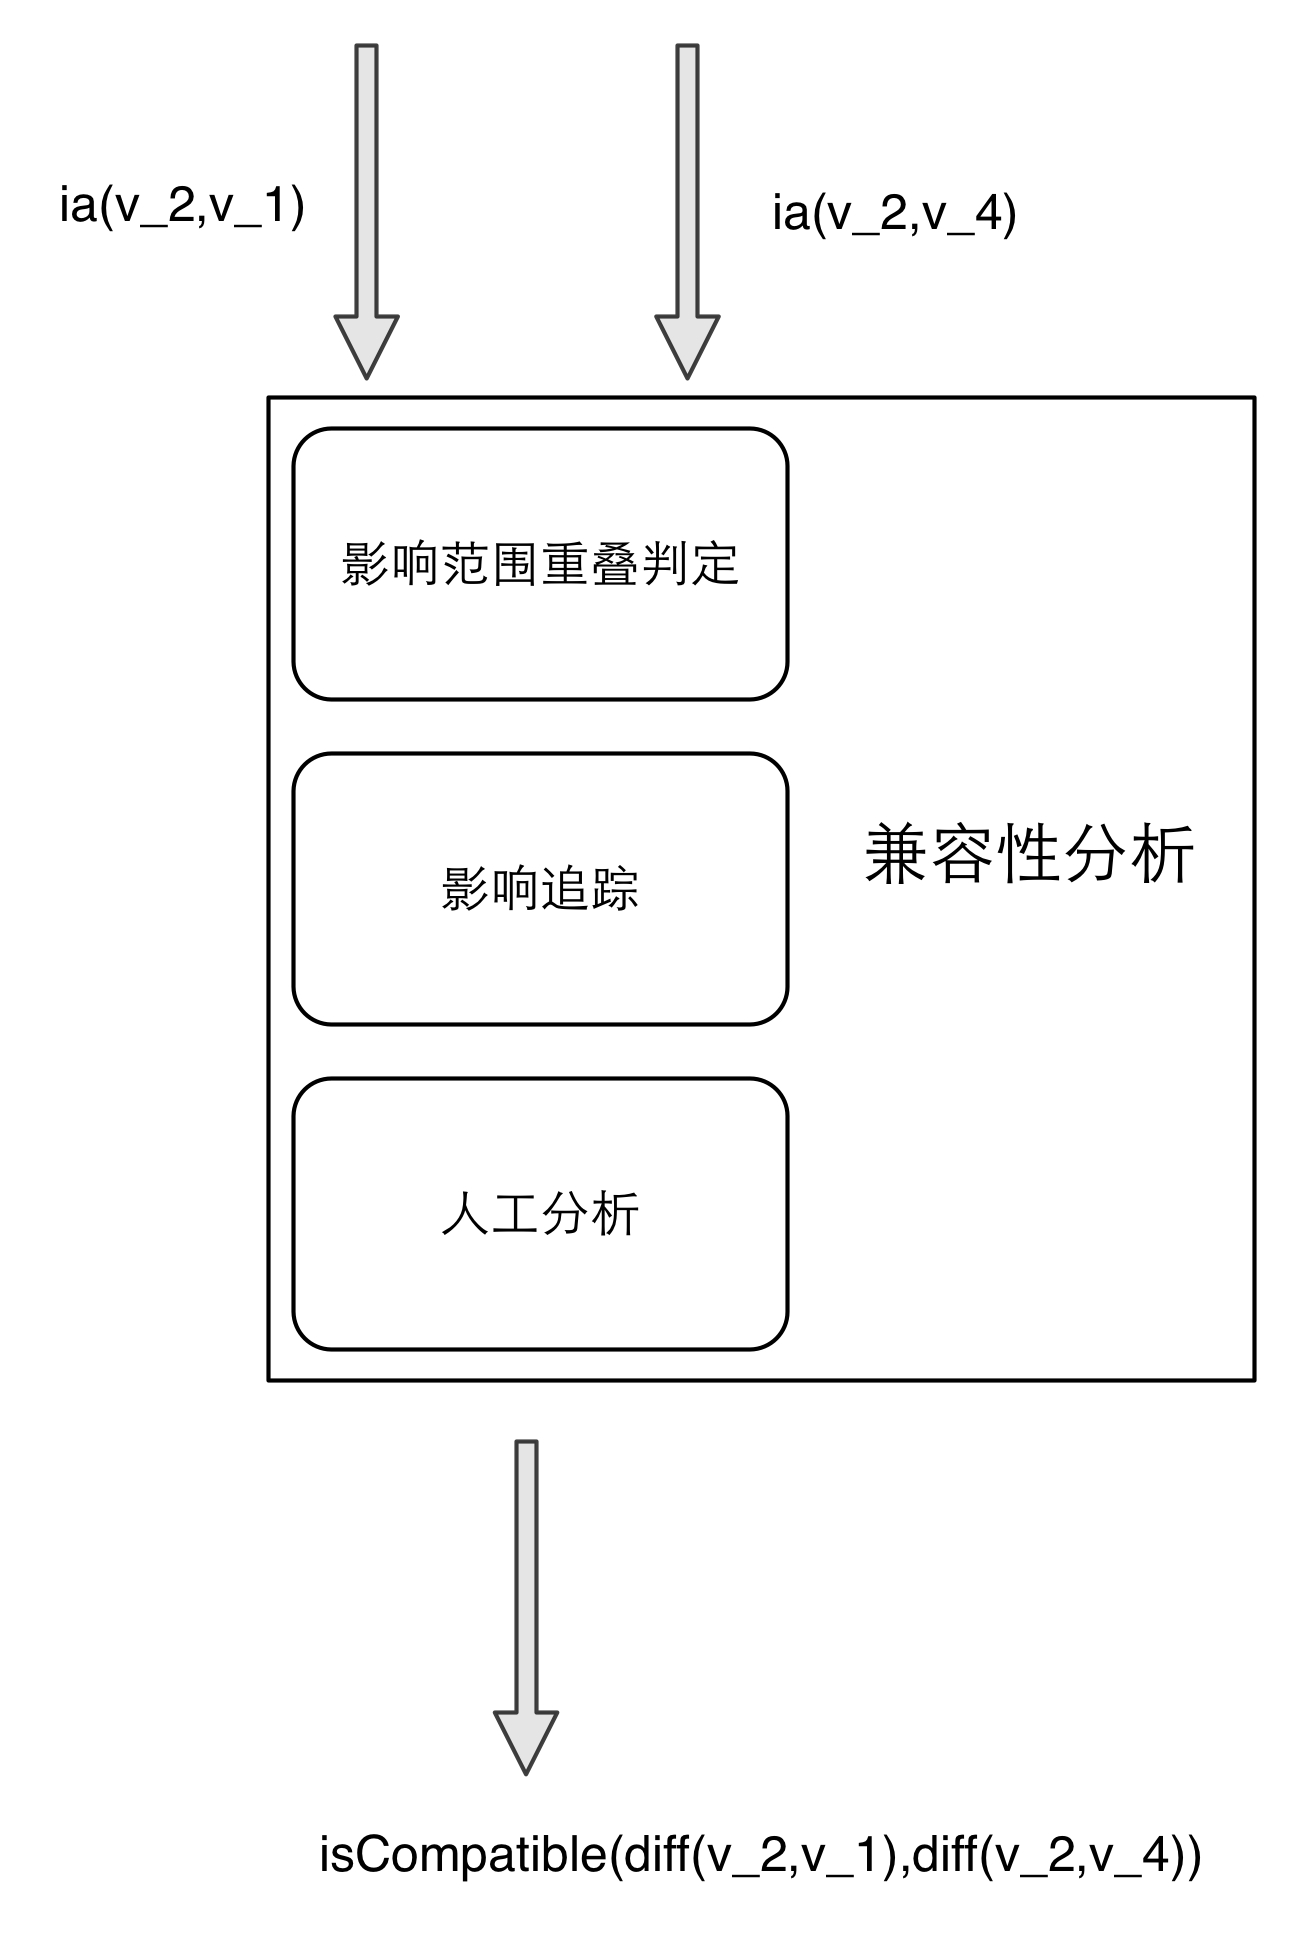
\includegraphics{chap03_isCompatible}
	\caption {兼容性分析}
	\label {isCompatible}	
\end{figure}

\subsection{整体流程}

根据前三节中给出的解决方案,我们将之整合,可以得到一个整体的解决方案和其解决流程。

其整体流程可以简述如下:

	\begin{enumerate}
		\item 采用git进行代码版本管理,并进行补丁版本迁移,得到应用于新版本的补丁后代码版本。
		\item 根据得到的三个版本代码,分别采用ASTro分析其程序间差异性,生成对应的程序变更集合。
		\item 根据得到的程序变更集合,采用jpf-regression进行不同版本间的变更影响分析,生成程序影响集合。
		\item 对得到的影响范围求交集以计算是否重叠,若不重叠,则说明兼容。若存在重叠的影响范围,进一步采用人工分析,确认是否确实不兼容。
	\end{enumerate}
	
	【此时可给出一张具体的流程图】
